
\section{Computer Algebra Representation}
\label{sec:car}

\rev{We use a computer algebra representation for working with the $P_N$-equations. It represents the equations using a tree of mathematical expressions, which represent numbers, symbols and other expression types, such as integrals, derivatives, sums, products and functions. Further, manipulators can be executed on these expression trees to perform substitution, constant folding, reordering of nested integrals, application of identities and more complex operations. Finally, frontends allow rendering the expression tree into different forms, such as \LaTeX~and C++ source code. While we ended up implementing our own lightweight framework, off-the-shelf packages, such as SymPy (www.sympy.org), exist and would be equally suitable for our use case.}

\begin{figure}[h]
%\vspace{1in}
\centering
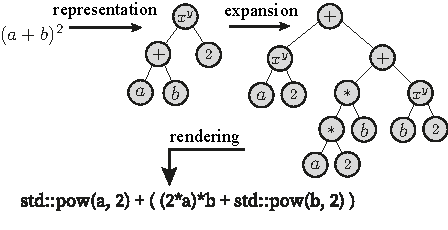
\includegraphics[width=0.9\columnwidth]{figures/fig_car_small.pdf}
%\missingfigure{figures fig car}
\vspace{-0.16in}
\icaption{\rev{A} computer algebra framework allows to represent equations as mathematical expressions trees. It further provides a set of functions for manipulating the tree according to valid mathematical operations, such as the binomial expansion above. Frontends allow generation of source code from the expression tree.}
\label{fig:staggeredgrid}
\end{figure}

\rev{Using the computer algebra representation, we perform the derivation steps required to arrive at the real-valued $P_N$-equations (the derivation steps shown in the supplemental material were almost all rendered from the expression tree). More importantly, we use the representation to perform the discretization and generate the stencil code used by our solver. This is detailed in section~\ref{sec:solver_precomputation}}.





